\defcatagory{Waves}

\begin{question}%
  \qtitle{State what is meant by the \term{amplitude} of a wave}\qpoint{1}

  the maximum \refterm{displacement}~\hfill\point{1}

  \begin{tikzpicture}[scale=1.5]
    \path[->, thick, draw] (-0.5, 0) -- (5.5, 0);
    \path[->, thick, draw] (0, -1.5) -- (0, 1.5);
    \begin{scope}
      \clip (-0.5, -1) rectangle (5.5, 1);
      \path[thin, draw] (-1, -1) cos (0, 0) sin (1, 1) cos (2, 0) sin (3, -1) cos (4, 0) sin (5, 1) cos (6, 0);
    \end{scope}
    \path[thick, >={Triangle[]}, |<->|, draw] (1, 0) -- (1, 1) node[midway, label={[fill=white]right:amplitude}] {};
    \path[thick, >={Triangle[]}, |<->|, draw, not] (3, -1) -- (3, 1) node[midway, label={[fill=white, text=not]below right:\NOT this}] {};
    \path[dashed, thin, draw, not] (3, 1) -- (5, 1);
  \end{tikzpicture}
\end{question}

\begin{question}%
  \qtitle{State what is meant by the \term{displacement} of a wave}\qpoint{1}

  the distance from the equilibrium position / undisturbed position / midpoint / rest position~\hfill\point{1}
\end{question}

\begin{question}%
  \qtitle{\termnoindex[frequency]{Frequency}\index{frequency}\ldots}

  Def: the number of wavefronts / crests / \refterm{wavelength} passing a (fixed) point on the wave per unit time \OR number of oscillations of the source per unit time.\\*
  \NOT something per \textit{second}. See the NOTs under \refterm{velocity} \\*
  \NOT the number of \textit{complete} oscillations per unit time since frequency is not necessary an integer value.

  Quantity: $\text{\refterm{period}}\ ^{-1}$

  Unit: \SI{}{Hz} = \SI{}{s^{-1}}

  Not to be confused with \refterm{period} or \refterm{wavelength}.
\end{question}

\begin{question}%
  \qtitle{\termnoindex[period]{Period}\index{period}\ldots}

  Def: time between adjacent wavefronts \OR time for one oscillation.

  Quantity: $\text{\refterm{frequency}}\ ^{-1}$

  Unit: \SI{}{s}

  Not to be confused with \refterm{frequency} or \refterm{wavelength}.
\end{question}

\begin{question}%
  \qtitle{State the difference between a \term{stationary wave} and a \term{progressive wave} in terms of\ldots}

  \begin{itemize}
    \item [(i)] the energy transfer along the wave:\qpoint{1}
      
      in a stationary wave \refterm{energy} is not transferred \OR in a progressive wave \refterm{energy} is transferred~\hfill\point{1}

    \item [(ii)] the phase of two adjacent vibrating particles:\qpoint{1}

      in a stationary wave (adjacent) particles are \refterm{in phase} \OR in a progressive wave (adjacent) particles are \refterm{out of phase}/have a \refterm{phase difference}/not in phase~\hfill\point{1}

    \item [(iii)] the amplitude of the particles' vibration:\qpoint{1}

      in a progressive wave all particles have same amplitude \OR in a stationary wave nodes have minimum / zero amplitude and antinodes have maximum amplitude
        (or simply `amplitude varies for stationary wave')~\hfill\point{1}
  \end{itemize}

  \textbf{Note}: `Progressive wave being formed by one / stationary wave being formed by two waves' is \NOT a difference and is actually not correct.
\end{question}

\begin{question}%
  \qtitle{State what is meant by an \term{antinode} of the \refterm{stationary wave}}\qpoint{1}

  Position where maximum \refterm{amplitude}~\hfill\point{1}
\end{question}

\begin{question}%
  \qtitle{By reference to vibrations of the points on a wave and to its direction of energy transfer, distinguish between \term{transverse waves} and \term{longitudinal waves}.}\qpoint{2}

  Transverse waves have vibrations / displacement of particles that are perpendicular to the direction of energy travel / propagation~\hfill\point{1}\\*
  Longitudinal waves have vibrations / displacement of particles that are parallel to the direction of energy travel / propagation~\hfill\point{1}\\*
  \NOT direction of motion of the wave / wave travel
\end{question}

\begin{question}%
  \qtitle{State the conditions required for the formation of a \refterm{stationary wave}}\qpoint{2}

  (two) waves travelling (at same speed) in opposite directions overlap~\hfill\point{1}\\*
  waves (are same type and) have same \refterm{frequency}/\refterm{wavelength}~\hfill\point{1}
\end{question}

\begin{question}%
  \qtitle{Describe the features that are seen on the stretched string that indicate \refterm{stationary wave}s have been produced.}\qpoint{1}

  points on string have different \textbf{amplitudes} varying from maximum to zero/minimum~\hfill\point{1}
\end{question}

\begin{question}%
  \qtitle{Explain how \refterm{stationary wave}s are formed in a tube with one end closed / with a \refterm{microwave} source and a metal reflector (figure~\ref{fig:stat-metal-reflect}).}\qpoint{2}

  waves \textbf{from source} (e.g.\ loudspeaker) (travel down tube and) are reflected at closed end / reflector~\hfill\point{1}\\*
  two waves (travelling) in opposite directions with same \refterm{frequency}/\refterm{wavelength} and \refterm{speed} \reftermnoindex[superposition]{overlap}~\hfill\point{1}
\end{question}

\begin{figure}[h]%
  \figureruletop

  \begin{tikzpicture}[thick]
    \coordinate (source) at (2, 0);
    \coordinate (detector) at (9, 0);
    \coordinate (reflector) at (13, 0);

    \path[fill, opacity=0.5] (0, 0) rectangle (15, -1);
    \path[draw] (0, 0) -- (15, 0);

    \path[draw] (source) rectangle +(1.5, 2) node [anchor=center] (tip) {} node[midway, anchor=center] {source};
    \path[draw] ($(tip) - (0, 0.2em)$) +(0, -0.2em) -- +(1em, 0) -- +(1em, -1em) -- +(0, -0.8em);

    \begin{scope}[shift=(detector)]
      \path[draw] (-0.5, 0.2) rectangle (0.5, 0);
      \path[draw] (-0.05, 0.2) -- (-0.05, 1.6) -- (0.05, 1.6) -- (0.05, 0.2);
      \path[draw, fill=white] (0, 1.6) circle[radius=0.5em] node[above=1em] {detector $D$};
    \end{scope}

    \begin{scope}[shift=(reflector)]
      \path[draw, ultra thick] (0, 0) -- (0, 2) node[pos=0.7, anchor=center] (a) {};
      \path[draw, thick] (a.center) -- (1, 3) node[pos=1, above right] {metal reflector};
    \end{scope}
  \end{tikzpicture}

  \caption{Figure for question~\ref{q:stat-metal-reflect}}
  \label{fig:stat-metal-reflect}

  \figureruletbottom
\end{figure}

\begin{question}%
  \label{q:stat-metal-reflect}%
  \qtitle{Explain how $D$ is used to show that stationary waves are formed between reflector and wave source in figure~\ref{fig:stat-metal-reflect}}\qpoint{2}

  detector/$D$ is moved between reflector and source\hfill\point{1}\\*
  maximum, minimum/zero, (maximum… etc.) observed on meter\allowbreak/deflections\allowbreak/readings\allowbreak/measurements\allowbreak/recordings\hfill\point{1}\\*
  \NOT \refterm{node}s and \refterm{antinode}s observed.
\end{question}

\begin{question}%
  \qtitle{Describe the \term{Doppler effect}}\qpoint{1}

  \textbf{observed} \refterm{frequency} is different to source \refterm{frequency} when source moves relative to observer~\hfill\point{1}\\*
  \NOT due to change in position of source
\end{question}

\begin{question}%
  \qtitle{Describe what is meant by a \term{polarised wave}}\qpoint{2}

  vibrations are in a single direction~\hfill\point{1}\\*
  applies to transverse waves \OR normal to direction of wave energy travel / propagation~\hfill\point{1}\\*
  \NOT vibration in only one plane
\end{question}

\begin{question}%
  \qtitle{Use the principle of \refterm{superposition} to explain \textit{<some observation>}}\qpoint{2}

  the waves (that overlap) have \refterm{phase difference} of $x \si{\degree}$ / $y\ \si{rad}$ / path difference of $z \lambda$~\hfill\point{1}\\*
    constructive / destructive interference \OR displacement larger / smaller (depend on question)~\hfill\point{1}
\end{question}

\begin{question}%
  \qtitle{State what is meant by the \term{diffraction} of a wave.}\qpoint{2}

  When wave incident on/passes by/through an aperture/edge~\hfill\point{1}\\*
  it spreads (into the geometrical shadow)~\hfill\point{1}\\*
  \NOT bending\\*
  \NOT when the wave passes through an obstacle
\end{question}

\begin{question}%
  \qtitle{State what is meant by \term{interference} / \term{superposition}}\qpoint{2}

  when two (or more) waves \refterm{superpose}/meet/overlap~\hfill\point{1}\\*
  resultant displacement is the sum of the displacement of each wave~\hfill\point{1}\\*

  {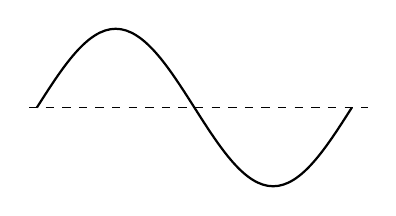
\begin{tikzpicture}[baseline=(a.center)]
    \path[thin, dashed, draw] (-0.1, 0) -- (4.2, 0);
    \path[thick, draw] (0, 0) sin (1, 1) cos (2, 0) sin (3, -1) cos (4, 0) node[pos=1, anchor=center] (a) {};
  \end{tikzpicture} \hfill $+$ \hfill 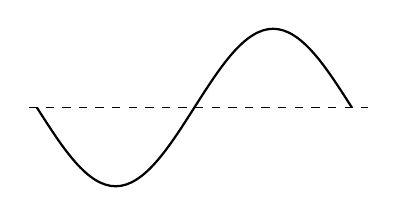
\begin{tikzpicture}[baseline=(a.center)]
    \path[thin, dashed, draw] (-0.1, 0) -- (4.2, 0);
    \path[thick, draw] (0, 0) sin (1, -1) cos (2, 0) sin (3, 1) cos (4, 0) node[pos=1, anchor=center] (a) {};
  \end{tikzpicture} \hfill $=$ \hfill 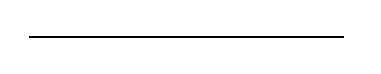
\begin{tikzpicture}[baseline=(a.center)]
    \path[thick, draw] (0, 0) -- (4, 0) node[pos=1, anchor=center] (a) {};
  \end{tikzpicture}}
\end{question}

\begin{question}%
  \qtitle{Explain the meaning of \term{coherent}}\qpoint{1}

  constant \refterm{phase difference}~\hfill\point{1}
\end{question}

\begin{question}%
  \qtitle{Explain the part played by \refterm{diffraction} in the production of the fringes in the \refterm{double slit experiment}}\qpoint{2}

  waves at (each) slit/aperture spread (into the geometric shadow)~\hfill\point{1}\\*
  (the spread) wave(s) overlap/\refterm[superposition]{superpose}/sum/meet/intersect~\hfill\point{1}
\end{question}

\begin{question}%
  \qtitle{Explain the reason why a double slit is used rather than two separate sources of light in the \refterm{double slit experiment}}\qpoint{1}

  two separate light sources are not in constant phase difference/\reftermnoindex[coherent]{coherence}\index{coherent}~\hfill\\*
  \OR waves/light from the double slit are \refterm{coherent}/have a constant phase difference~\hfill\point{1}
\end{question}

\begin{figure}[h]
  \figureruletop
  \centering\begin{tikzpicture}[baseline=(baseline.base)]
    \def\lightarrow#1{\path [draw, -{Stealth}, thick] (0, #1) -- (3, #1)}
    \lightarrow{1};
    \lightarrow{0.5}
      node[pos=1, anchor=base west, xshift=1em] (slitline1) {};
    \lightarrow{0}
      node[midway, anchor=base east, align=right, fill=white] (baseline) {laser light}
      node[pos=1, anchor=base west, xshift=1em] (centerline) {};
    \lightarrow{-0.5}
      node[pos=1, anchor=base west, xshift=1em] (slitline2) {};
    \lightarrow{-1};

    \path [draw=black, fill=gray, thick] ([yshift=0.25em, xshift=-0.25em]slitline1) rectangle ([yshift=3.25em, xshift=0.25em]slitline1) node[pos=1, anchor=west] (top) {};
    \path [draw=black, fill=gray, thick] ([yshift=-0.25em, xshift=-0.25em]slitline1) rectangle ([yshift=0.25em, xshift=0.25em]slitline2);
    \path [draw=black, fill=gray, thick] ([yshift=-0.25em, xshift=-0.25em]slitline2) rectangle ([yshift=-3.25em, xshift=0.25em]slitline2) node[pos=1, anchor=west] (bottom) {};
    \path [draw=black, thick, dashed] ([xshift=0.5em]centerline) -- ++ (12em, 0) node[pos=1, anchor=base west] (lineright) {};

    \def\letterbox#1{\makebox[1em][l]{#1}}

    \path [draw, thick] let \p1 = (lineright), \p2 = (top), \p3 = (bottom) in (\x1, \y2) -- (\x1, \y3)

      node[midway, right, align=left] {\letterbox{$X$} (centeral bright fringe)}
      node[midway, anchor=center, shape=circle, inner sep=0.2em, fill=black, draw=none] {}

      node[pos=0.25, right, align=left] {\letterbox{$Y$} (a dark fringe)}
      node[pos=0.25, anchor=center, shape=circle, inner sep=0.2em, fill=gray, draw=none] {}

      node[pos=0.75, right, align=left] {\letterbox{$Z$} (another dark fringe)}
      node[pos=0.75, anchor=center, shape=circle, inner sep=0.2em, fill=gray, draw=none] {};
  \end{tikzpicture}

  \caption{for question~\ref{q:double-slits-q1} and~\ref{q:double-slits-q2}. Not to scale.}
  \label{fig:double-slits-x}
  \figureruletbottom
\end{figure}

\begin{question}%
  \label{q:double-slits-q1}%
  \qtitle{Explain why a bright fringe is produced at point $X$ in figure~\ref{fig:double-slits-x}.}\qpoint{2}

  waves (from slits) overlap (at point $X$)~\hfill\point{1}

  path difference (from slits to $X$) is zero\\*
  \OR phase difference (between the two waves) is zero~\hfill\point{1}\\*
  (so constructive interference gives bright fringe)

  \NOT statements that applies to all bright fringes in general -- e.g. path difference = $n \lambda$ or
  phase difference = $\SI{360}{\degree} n$.
\end{question}

\begin{question}%
  \label{q:double-slits-q2}%
  \qtitle{The intensity of the light passing through the two slits in figure~\ref{fig:double-slits-x} was initially
    the same. The intensity of the light through one of the slits is now reduced. Compare the appearance of the fringes before and after the change of intensity.}\qpoint{2}

  Any \point{2} of:\\*
  same separation/fringe width/number of fringes\\*
  bright fringes/central bright fringe/(fringe at) $X$ less bright\\*
  dark fringes/(fringe at) $Y$/$Z$ brighter

  \NOT `fringes' if it is not clear whether it refers to the dark fringes or the white fringes.
\end{question}

\begin{question}%
  \qtitle{Describe the \refterm{diffraction} of light at a \refterm{diffraction grating}}\qpoint{2}

  waves at the slits \point{1} spread (into the geometric shadow) \point{1}\\*
  \NOT light spread without the word `wave'
\end{question}

\begin{question}%
  \label{q:dffgrat-d-and-i-first}%
  \qtitle{Explain the part played by \refterm{diffraction} and \refterm[superposition]{interference} in the production of the first order maximum by the \refterm{diffraction grating}.}\qpoint{3}

  diffraction: spreading/diverging of waves/light (takes place) at (each) slit\allowbreak/element\allowbreak/gap\allowbreak/aperture~\hfill\point{1} \\*
  interference: waves (from \refterm{coherent} sources at each slit) overlap \point{1} with phase difference \SI{360}{\degree} / path difference $\lambda$ \point{1}

  See also: question~\ref{q:dffgrat-zero-and-first}
\end{question}

\begin{question}%
  \label{q:dffgrat-zero-and-first}%
  \qtitle{By reference to \refterm[superposition]{interference}, explain the zero and first order maximum in a \refterm{diffraction grating}.}\qpoint{3}

  \begin{itemize}
    \item[zero:] waves (from each slit) overlap/meet/\refterm[superposition]{superpose} \point{1} with a phase difference/path difference of zero \point{1}
    \item[first:] phase difference is \SI{360}{\degree}/path difference of $\lambda$~\hfill\point{1}
  \end{itemize}

  For the first mark, explicit mentioning that the waves \textbf{meet} or otherwise interference is necessary.

  See also: question~\ref{q:dffgrat-d-and-i-first}
\end{question}
